	\documentclass[xcolor={dvipsnames,table},aspectratio=169]{beamer}
\usepackage[utf8]{inputenc}
\usepackage[T1]{fontenc}
\usepackage[brazil]{babel}
\usepackage{graphics,amssymb,amsfonts,amsmath}
\usepackage{tikz}
\usepackage{enumerate,hyperref}
\usepackage{palatino}
\usepackage{ragged2e}
\usepackage{minted}
\usepackage{booktabs}
\usepackage{verbatim}
\usepackage[export]{adjustbox}
\usepackage{xcolor}
\usepackage{textcomp} % para usar \textdegree
\usetikzlibrary{shadows}
\usetheme{AnnArbor}
\usecolortheme{orchid}
\usefonttheme[onlymath]{serif}

\newcommand\setItemnumber[1]{\setcounter{enumi}{\numexpr#1-1\relax}}

\AtBeginSection[]{
  \begin{frame}
  \vfill
  \centering
  \begin{beamercolorbox}[sep=8pt,center,shadow=true,rounded=true]{title}
    \usebeamerfont{title}\insertsectionhead\par%
  \end{beamercolorbox}
  \vfill
  \end{frame}
}

\newminted{java}{bgcolor=cyan!10}

\newcolumntype{C}[1]{>{\centering\let\newline\\\arraybackslash\hspace{0pt}}m{#1}}

\title[\sc{Objetos e Classes}]{Objetos e Classes}
\author[Roland Teodorowitsch]{Roland Teodorowitsch}
\institute[FPROG - EP - PUCRS]{Fundamentos de Programação - Escola Politécnica - PUCRS}
\date{13 de junho de 2023}

\begin{document}
\justifying

%-------------------------------------------------------
\begin{frame}
	\titlepage
\end{frame}

%=======================================================
\section{Introdução}

%-------------------------------------------------------
\begin{frame}\frametitle{Objetivos}
\begin{itemize}
	\item Entender os conceitos de classes, objetos e encapsulamento
	\item Implementar variáveis, métodos e construtores de instância
	\item Ser capaz de projetar, implementar e testar classes
	\item Entender o compartamento de referências a objetos, variáveis estáticas e métodos estáticos
\end{itemize}
\end{frame}

%-------------------------------------------------------
\begin{frame}\frametitle{Conteúdos}
\begin{itemize}
	\item Programação Orientada a Objetos
	\item Implementando uma Classe Simples
	\item Construtores
	\item Exemplos
	\item Passos para Implementar uma Classe

	\item Testando uma Classe
	\item Padrões para Dados de Objetos
	\item Referências a Objetos
	\item Variáveis e Métodos Estáticos
	\item Sumário
	\item Tópicos Complementares
\end{itemize}
\end{frame}

%=======================================================
\section{Programação Orientada a Objetos}

%-------------------------------------------------------
\begin{frame}\frametitle{Programação Orientada a Objetos}
\begin{itemize}
	\item Até agora foram apresentadas técnicas de programação estruturada
	\begin{itemize}
		\item Quebrar tarefas em subtarefas
		\item Escrever métodos reusáveis para tratar tarefas
	\end{itemize}
	\item A partir de agora serão estudados objetos e classes
	\begin{itemize}
		\item Para construir programas maiores e mais complexos
		\item Para modelar objetos que são usados no mundo real
	\end{itemize}
\end{itemize}
\begin{block}{Classes e Objetos}
Uma classe descreve objetos com um comportamento comum.
Por exemplo, a classe Carro descreve todos os veículos de passageiros que tem determinada capacidade e formato.
\end{block}
\end{frame}

%-------------------------------------------------------
\begin{frame}[fragile]\frametitle{Objetos e Programas}
\begin{itemize}
	\item Programas Java são feitos por objetos que interagem uns com os outros
	\begin{itemize}
		\item Cada objeto é baseado em uma classe
		\item Uma classe descreve um conjunto de objetos o mesmo comportamento 
	\end{itemize}
	\item Cada classe define um conjunto específico de métodos para ser usado com os seus objetos
	\begin{itemize}
		\item Por exemplo, a classe \texttt{String} provê métodos tais como \texttt{length()} e \texttt{charAt()}
		\item Estes métodos foram definidos na classe \texttt{String} e podem ser usados por qualquer objeto desta classe
	\end{itemize}
\end{itemize}
\begin{javacode}
String boasVindas = "Sejam bem-vindos!";
int  tamanho = boasVindas.length();
char caract1 = boasVindas.charAt(0);
\end{javacode}
\end{frame}

%-------------------------------------------------------
\begin{frame}\frametitle{Diagrama de Classes}
\begin{columns}[T]
	\begin{column}{0.7\linewidth}
\begin{itemize}
	\item Dados Privados
	\begin{itemize}
		\item Cada objeto tem seus próprios dados privados que outros objetos não podem acessar diretamente
		\item Métodos da interface pública provêm acesso a dados privados, enquanto escondem detalhes de implementação
		\item Isto é chamado de \textbf{encapsulamento}
	\end{itemize}
	\item Interface Pública
	\begin{itemize}
		\item Cada objeto tem um conjunto de métodos disponível para ser usado por outros objetos
	\end{itemize}
\end{itemize}
	\end{column}
	\begin{column}{0.3\linewidth}
\begin{figure}[h]
	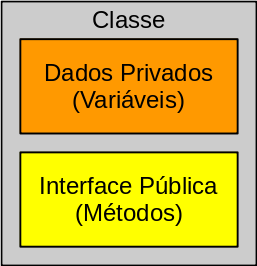
\includegraphics[height=0.4\paperheight,center]{pucrs-ep-fprog-unidade_07-objetos_e_classes-laminas-diagrama_de_classes.png}
\end{figure}
	\end{column}
\end{columns}
\end{frame}

%-------------------------------------------------------
\begin{frame}\frametitle{Tipos Abstratos de Dados}
\begin{itemize}
	\item \textbf{Abstração} é uma visão ou representação de uma entidade que inclui apenas os seus atributos mais importantes segundo determinado ponto de vista
	\begin{itemize}
		\item Em Computação, usa-se a abstração para atenuar a complexidade de problemas
	\end{itemize}
	\item Um \textbf{Tipo Abstrato de Dados} (TAD) é uma estrutura sintática que define um tipo para determinada entidade, de forma que quem o usa não necessite conhecer os detalhes da sua implementação (armazenamento interno de dados ou implementação de operações suportadas)
	\begin{itemize}
		\item TADs são importantes para garantir encapsulamento
	\end{itemize}
	\item \textbf{Encapsulamento} é uma técnica que agrupa elementos relacionados entre si (tipos, variáveis, métodos, etc.) em um módulo, escondendo do usuário seus detalhes internos, o que garante abstração
	\begin{itemize}
		\item O encapsulamento define quais partes de um objeto serão visíveis (públicas) e quais partes permanecerão ocultas (privadas)
	\end{itemize}
	\item Em Java, classes são usadas para a criação de Tipos Abstratos de Dados
\end{itemize}
\end{frame}

%=======================================================
\section{Implementando uma Classe Simples}

%-------------------------------------------------------
\begin{frame}\frametitle{Implementando uma Classe Simples}
\begin{itemize}
	\item Exemplo: contador\\Uma classe que modela um dispositivo mecânico que é usado para realizar contagens
	\begin{itemize}
		\item Por exemplo, para contar quantas pessoas estão assistindo a um concerto ou quantas pessoas embarcaram em um ônibus
	\end{itemize}
\begin{figure}[h]
	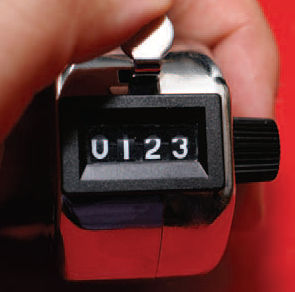
\includegraphics[height=0.25\paperheight,center]{pucrs-ep-fprog-unidade_07-objetos_e_classes-laminas-tally_counter.jpg}
\end{figure}
	\item O que deve ser feito?
	\begin{itemize}
		\item Inicializar o contador (Java já faz isso automaticamente...)
		\item Incrementar o dispositivo
		\item Obter o valor atual
	\end{itemize}
\end{itemize}
\end{frame}

%-------------------------------------------------------
\begin{frame}\frametitle{Classe \texttt{Contador}}
\begin{itemize}
	\item Especifica-se variáveis de instância na declaração da classe:
\begin{figure}[h]
	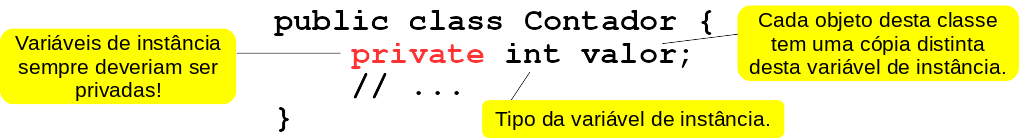
\includegraphics[height=0.2\paperheight,center]{pucrs-ep-fprog-unidade_07-objetos_e_classes-laminas-classe_contador.png}
\end{figure}
	\item Cada objeto instanciado a partir desta classe terá seu próprio conjunto de variáveis de instância
	\begin{itemize}
		\item Cada objeto da classe \texttt{Contador} terá sua própria variável \texttt{valor}
	\end{itemize}
	\item Especificadores de acesso
	\begin{itemize}
		\item Classes (e métodos de interface) são públicos (\texttt{public})
		\item Variáveis de instância são privadas (\texttt{private})
	\end{itemize}
\end{itemize}
\end{frame}

%-------------------------------------------------------
\begin{frame}[fragile]\frametitle{Instanciando Objetos}
\begin{columns}[T]
	\begin{column}{0.55\linewidth}
\begin{itemize}
	\item Objetos são criados a partir de classes
	\begin{itemize}
		\item Usa-se o operador \texttt{new} para construir objetos
		\item Cada objeto recebe um nome único (da mesma forma que uma variável)
	\end{itemize}
	\item O operador \texttt{new} já apareceu em exemplos anteriores
{\scriptsize
\begin{javacode}
Scanner in = new Scanner(System.in);
\end{javacode}
}
	\item Para criar duas instâncias de objetos da classe \texttt{Contador}, usa-se:
{\scriptsize
\begin{javacode}
// NomeClasse nomeObjeto = new NomeClasse();
Contador presentes  = new Contador();
Contador embarcaram = new Contador();
\end{javacode}
}
\end{itemize}
	\end{column}
	\begin{column}{0.45\linewidth}
\begin{figure}[h]
	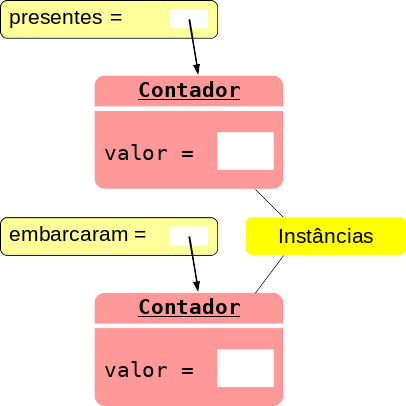
\includegraphics[height=0.60\paperheight,center]{pucrs-ep-fprog-unidade_07-objetos_e_classes-laminas-objetos_contador.png}
\end{figure}
	\end{column}
\end{columns}
\end{frame}

%-------------------------------------------------------
\begin{frame}[fragile]\frametitle{Métodos da Classe \texttt{Contador}}
\begin{columns}[T]
	\begin{column}{0.5\linewidth}
\begin{itemize}
	\item Dois métodos serão usados para acessar as variáveis de instância dos objetos da classe \texttt{Contador}
	\begin{itemize}
		\item \texttt{incrementaValor()}: incrementa o valor da variável de instância \texttt{valor}
		\item \texttt{obtemValor()}: retorna o valor da variável de instância \texttt{valor}
	\end{itemize}
	\item Para usar estes métodos, é preciso especificar sobre qual objeto eles deverão ser aplicados
{\scriptsize
\begin{javacode}
presentes.incrementaValor();
embarcaram.incrementaValor();
\end{javacode}
}	
\end{itemize}
	\end{column}
	\begin{column}{0.5\linewidth}
{\scriptsize\inputminted[bgcolor=cyan!10]{java}{src/contagem0/Contador.java}}
	\end{column}
\end{columns}
\end{frame}

%-------------------------------------------------------
\begin{frame}[fragile]\frametitle{Tipos de Métodos}
\begin{enumerate}
	\item Métodos de Acesso (\emph{Accessors} ou \emph{getters})
	\begin{itemize}
		\item Solicitam uma informação ao objeto sem alterá-lo
		\item Normalmente retornam algum valor
		\item Em inglês costumam iniciar com o prefixo \texttt{get}; em Português, \texttt{obtem}
	\end{itemize}
\begin{javacode}
public int obtemValor() { return valor }
\end{javacode}
	\item Métodos de Alteração (\emph{Mutators} ou \emph{setters})
	\begin{itemize}
		\item Alteram valores no objeto
		\item Geralmente recebem um parâmetro que será usado para alterar uma variável de instância
		\item Normalmente o tipo de retorno é \texttt{void}
		\item Em inglês costumam iniciar com o prefixo \texttt{set}; em Português, \texttt{define	}
	\end{itemize}
\begin{javacode}
public void incrementaValor() { ++valor; }
public void defineValor(int v) { valor = v; }
\end{javacode}
\end{enumerate}
\end{frame}

%-------------------------------------------------------
\begin{frame}[fragile]\frametitle{Métodos Estáticos x Não-Estáticos}
\begin{itemize}
	\item Quando um método (ou membro) é declarado como \texttt{static}, ele existe e pode ser acessado mesmo se nenhum objeto da classe for criado (lembre-se da classe \texttt{Math})
	\item Para métodos de instância (não-estáticos), é preciso instanciar um objeto da classe antes que o método possa ser invocado (lembre-se da classe \texttt{Scanner})
	\item Somente depois de criar um objeto, é possível invocar os seus métodos não-estáticos
	\item Métodos estáticos \textbf{SOMENTE} podem invocar métodos estáticos
	\item Métodos de instância podem acessar métodos estáticos
\end{itemize}
\begin{javacode}
Contador presentes = new Contador(); // Cria o objeto
presentes.incrementaValor(); // Invoca um de seus metodos
\end{javacode}
\end{frame}

%=======================================================
\section{Construtores}

%-------------------------------------------------------
\begin{frame}[fragile]\frametitle{Construtores}
\begin{itemize}
	\item Um construtor é um método que inicializa as variáveis de instância de um objeto
	\begin{itemize}
		\item Ele é automaticamente chamado quando um objeto é criado
		\item Ele tem exatamente o mesmo nome da classe
	\end{itemize}
	\item Construtores nunca retornam valores, mas \textbf{não se usa \texttt{void} na sua declaração}
\end{itemize}
{\scriptsize\inputminted[bgcolor=cyan!10]{java}{src/contagem1/Contador.java}}
\end{frame}

%-------------------------------------------------------
\begin{frame}[fragile]\frametitle{Múltiplos Construtores (Sobrecarga)}
\begin{itemize}
	\item Uma classe pode ter mais de um construtor, mas cada um tem que ter um conjunto único de parâmetros
{\tiny\inputminted[bgcolor=cyan!10]{java}{src/contagem2/Contador.java}}
	\item O compilador seleciona o construtor que corresponde aos parâmetros especificados na construção
{\tiny
\begin{javacode}
Contador presentes = new Contador(10);
Contador embarcaram = new Contador();
\end{javacode}
}
\end{itemize}
\end{frame}

%-------------------------------------------------------
\begin{frame}\frametitle{Sintaxe de Construtores}
\begin{itemize}
	\item Um construtor é invocado quando um objeto é criado com a palavra-reservada \texttt{new}
\end{itemize}
\begin{figure}[h]
	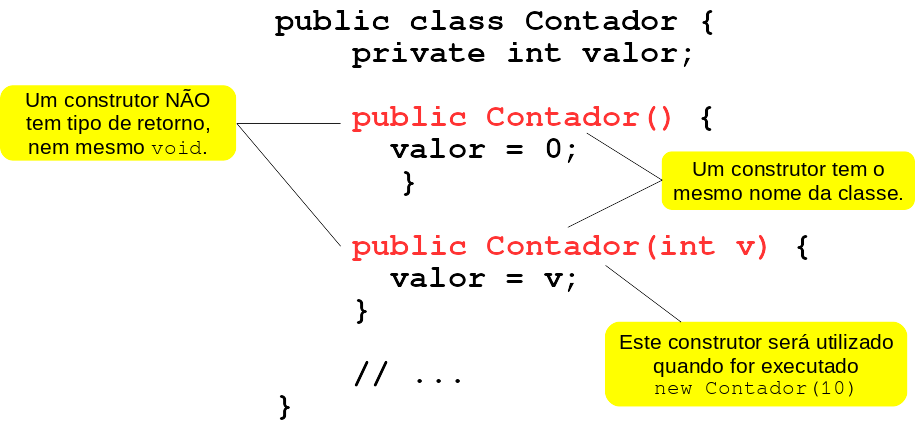
\includegraphics[height=0.60\paperheight,center]{pucrs-ep-fprog-unidade_07-objetos_e_classes-laminas-sintaxe_construtores.png}
\end{figure}
\end{frame}

%-------------------------------------------------------
\begin{frame}[fragile]\frametitle{O Construtor Padrão}
\begin{itemize}
	\item Se nenhum construtor for declarado, o compilador criará um construtor padrão automaticamente
	\begin{itemize}
		\item Ele não receberá nenhum parâmetro
		\item Ele inicializará todas as variáveis de instância
		\item Números são inicializados com 0, booleanos com \texttt{false} e objetos com \texttt{null}
	\end{itemize}
\end{itemize}
{\scriptsize\inputminted[bgcolor=cyan!10]{java}{src/contagem1/Contador.java}}
\end{frame}

%=======================================================
\section{Exemplos}

%-------------------------------------------------------
\begin{frame}[fragile]\frametitle{Classe com \texttt{main()}: \texttt{Contador.java}}
{\tiny\inputminted[bgcolor=cyan!10]{java}{src/contagem3/Contador.java}}
\end{frame}

%-------------------------------------------------------
\begin{frame}[fragile]\frametitle{Duas Classes no mesmo Arquivo: \texttt{TestaContador.java}}
{\tiny\inputminted[bgcolor=cyan!10]{java}{src/contagem4/TestaContador.java}}
\end{frame}

%-------------------------------------------------------
\begin{frame}[fragile]\frametitle{Classes em Arquivos Separados: \texttt{Contador.java}}
{\tiny\inputminted[bgcolor=cyan!10]{java}{src/contagem5/Contador.java}}
\end{frame}

%-------------------------------------------------------
\begin{frame}[fragile]\frametitle{Classes em Arquivos Separados: \texttt{TestaContador.java}}
{\tiny\inputminted[bgcolor=cyan!10]{java}{src/contagem5/TestaContador.java}}
\end{frame}

%=======================================================
\section{Passos para Implementar uma Classe}

%-------------------------------------------------------
\begin{frame}[fragile]\frametitle{Passos para Implementar uma Classe}
\begin{enumerate}
	\item Crie uma lista informal de tarefas para os objetos: adicionar, obter, limpar, etc.
	\item Especifique a interface pública (por exemplo, para uma caixa registradora)
{\tiny
\begin{javacode}
void adicionaItem(double preco);    int obtemNumItems();    double obtemTotal();    	void limpa();
\end{javacode}
}
	\item Documente a interface pública com comentários Javadoc
{\tiny
\begin{javacode}
/** Adiciona um item na caixa registradora.
    @param preco Preço do item a ser registrado. */
\end{javacode}
}
	\item Determine as variáveis de instância
{\tiny
\begin{javacode}
private int numItens;                       private double total;
\end{javacode}
}
	\item Implemente os construtores e métodos
{\tiny
\begin{javacode}
public void adicionaItem(double preco) {  numItens++; total = total + preco; }
\end{javacode}
}
	\item Teste a classe
\end{enumerate}
\end{frame}

%-------------------------------------------------------
\begin{frame}\frametitle{Interface Pública de uma Classe}
\begin{itemize}
	\item Quando se projeta uma classe, um dos primeiros passos é especificar a sua \textbf{interface pública}
	\item Por exemplo: uma classe para uma caixa registradora
	\begin{itemize}
		\item Quais tarefas esta classe deverá executar?
		\item Que métodos serão necessários?
		\item Que parâmetros cada método receberá?
		\item O que os métodos retornarão?
	\end{itemize}
\end{itemize}
{\footnotesize
\begin{center}
\begin{tikzpicture}
\node[drop shadow,fill=white,inner sep=0pt] 
{\rowcolors{1}{RoyalBlue!20}{RoyalBlue!5}
  \begin{tabular}{|l|l|l|}
\hline
    \textbf{Tarefa} & \textbf{Método} & \textbf{Retorno}\\
\hline
Adiciona o preço de um item & \texttt{adicionaItem(double)}    & \texttt{void}\\
Obtém o total devido & \texttt{obtemTotal()}    & \texttt{double}\\
Obtém o número de itens comprados & \texttt{obtemNumItens()}    & \texttt{int}\\
Limpa o registro da caixa registradora para uma nova venda & \texttt{limpa()}    & \texttt{void}\\
\hline
  \end{tabular}
};
\end{tikzpicture}
\end{center}
}
\end{frame}

%-------------------------------------------------------
\begin{frame}[fragile]\frametitle{Escrevendo a Interface Pública de uma Classe}
\begin{itemize}
	\item É importante usar comentários no estilo Javadoc para documentar a classe e o funcionamento de cada método
	\item As declarações de métodos correspondem à interface pública da classe
	\item Os dados e o corpo dos métodos correspondem à implementação privada da classe
\end{itemize}
{\tiny
\begin{javacode}
/** Simula uma caixa registradora, com número de itens e valor total dos itens. */
public class CaixaRegistradora {

  /** Adiciona um item na caixa registradora.
      @param preco Preço do item a ser registrado. */
  public void adicionaItem(double preco) {
    numItens++;
    total = total + preco;
  }

  /** Obtém o valor total de todos os itens registrados.
      @return Valor total de todos os itens registrados. */
  public double obtemTotal() {
    return total;
  }

  // ...
\end{javacode}
}
\end{frame}

%-------------------------------------------------------
\begin{frame}[fragile]\frametitle{Javadoc}
\begin{columns}[T]
	\begin{column}{0.35\linewidth}
\begin{itemize}
	\item O utilitário \texttt{javadoc} gera um conjunto de arquivos HTML a partir dos comentários no estilo Javadoc
	\item Parâmetros e retornos de métodos devem ser descritos com as anotações \texttt{@param} e \texttt{@return}
\end{itemize}
{\scriptsize\texttt{~\\~\\javadoc CaixaRegistradora.java}}
	\end{column}
	\begin{column}{0.65\linewidth}
\begin{figure}[h]
	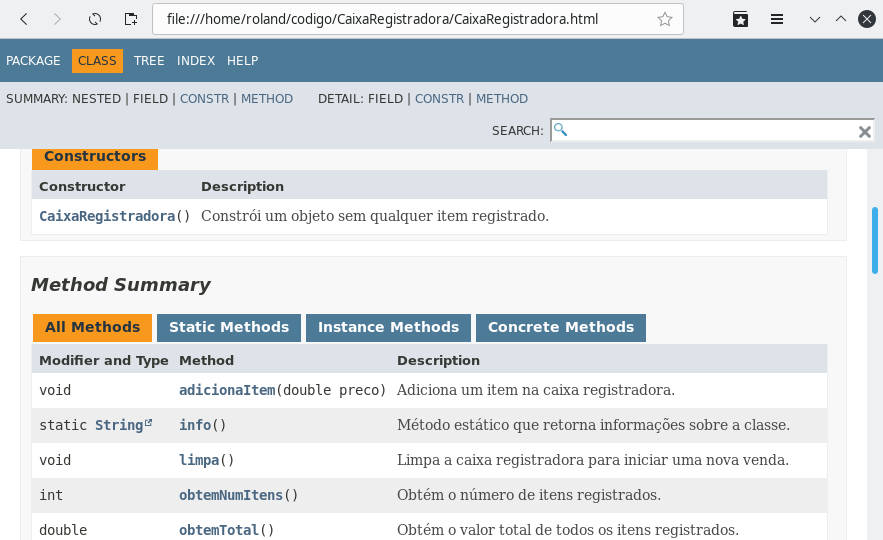
\includegraphics[height=0.65\paperheight,center]{pucrs-ep-fprog-unidade_07-objetos_e_classes-laminas-javadoc.jpg}
\end{figure}
	\end{column}
\end{columns}

\end{frame}

%-------------------------------------------------------
\begin{frame}[fragile]\frametitle{Projetando a Representação de Dados}
\begin{itemize}
	\item Um objeto armazena dados em variáveis de instância
	\begin{itemize}
		\item Variáveis de instância são declaradas dentro da classe e devem ser privadas
{\tiny
\begin{javacode}
/** Simula uma caixa registradora, com número de itens e valor total dos itens. */
public class CaixaRegistradora {
  private int numItems;
  private double total;
  // ...
\end{javacode}
}
		\item Todos os métodos (não estáticos) dentro da classe têm acesso a elas, podendo modificar os seus valores
		\item Quais dados os métodos da classe da caixa registradora necessitam?
	\end{itemize}
\end{itemize}
{\footnotesize
\begin{center}
\begin{tikzpicture}
\node[drop shadow,fill=white,inner sep=0pt] 
{\rowcolors{1}{RoyalBlue!20}{RoyalBlue!5}
  \begin{tabular}{|p{6cm}|l|p{3cm}|}
\hline
    \textbf{Tarefa} & \textbf{Método} & \textbf{Dado(s) necessário(s)}\\
\hline
Adiciona o preço de um item & \texttt{adicionaItem()}    & \texttt{total}, \texttt{numItens}\\
Obtém o \textbf{total} devido & \texttt{obtemTotal()}    & \texttt{total}\\
Obtém o \textbf{número de itens} comprados & \texttt{obtemNumItens()}    & \texttt{numItens}\\
Limpa o registro da caixa registradora para uma nova venda & \texttt{limpa()}    & \texttt{total}, \texttt{numItens}\\
\hline
  \end{tabular}
};
\end{tikzpicture}
\end{center}
}
\end{frame}

%-------------------------------------------------------
\begin{frame}\frametitle{Variáveis de Instância de Objetos}
\begin{itemize}
	\item Cada objeto de uma classe tem um conjunto exclusivo de variáveis de instância
	\item Os valores armazenados nas variáveis de instância constituem o estado do objeto
\begin{figure}[h]
	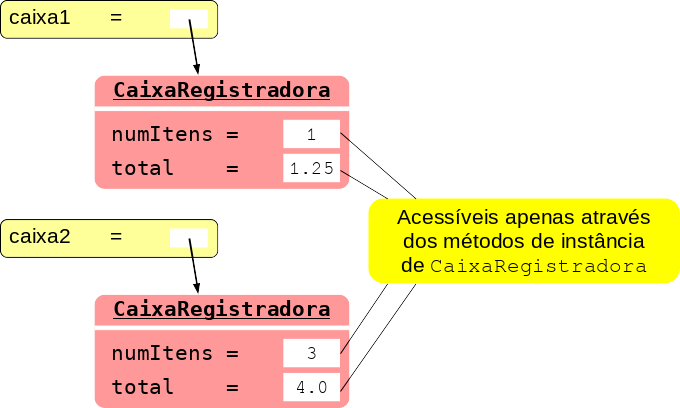
\includegraphics[height=0.55\paperheight,center]{pucrs-ep-fprog-unidade_07-objetos_e_classes-laminas-objetos_caixaregistradora.png}
\end{figure}
\end{itemize}
\end{frame}

%-------------------------------------------------------
\begin{frame}[fragile]\frametitle{Acessando Variáveis de Instância}
\begin{itemize}
	\item Variáveis de instância privadas (\texttt{private}) não podem ser acessadas de fora da classe: o compilador não permite esta violação de privacidade
{\footnotesize
\begin{javacode}
public static void main(String[] args) {
  CaixaRegistradora caixa1 = new CaixaRegistradora();
  System.out.println( caixa1.numItens ); // ERRO
}
\end{javacode}
}
	\item Em vez disto, usam-se métodos para acessar os dados da classe: o encapsulamento provê uma interface pública e esconde os detalhes de implementação
{\footnotesize
\begin{javacode}
public static void main(String[] args) {
  CaixaRegistradora caixa1 = new CaixaRegistradora();
  System.out.println( caixa1.obtemNumItens() ); // OK
}
\end{javacode}
}
\end{itemize}
\end{frame}

%-------------------------------------------------------
\begin{frame}[fragile]\frametitle{Implementando Métodos de Instância}
\begin{itemize}
	\item Métodos de instância acessam variáveis de instância privadas
\begin{javacode}
public void adicionaItem(double preco) {
  numItens++;
  total = total + preco;
}
\end{javacode}
	\item Métodos de instância
	\begin{itemize}
		\item São declarados dentro da classe como \texttt{public}
		\item Não há necessidade de especificar o nome do objeto (parâmetro implícito) quando se usa alguma variável de instância dentro de uma classe
		\item Os parâmetros explícitos (variáveis paramétricas) são listados na declaração do método
	\end{itemize}
\end{itemize}
\end{frame}

%-------------------------------------------------------
\begin{frame}\frametitle{Sintaxe de Métodos de Instância}
\begin{figure}[h]
	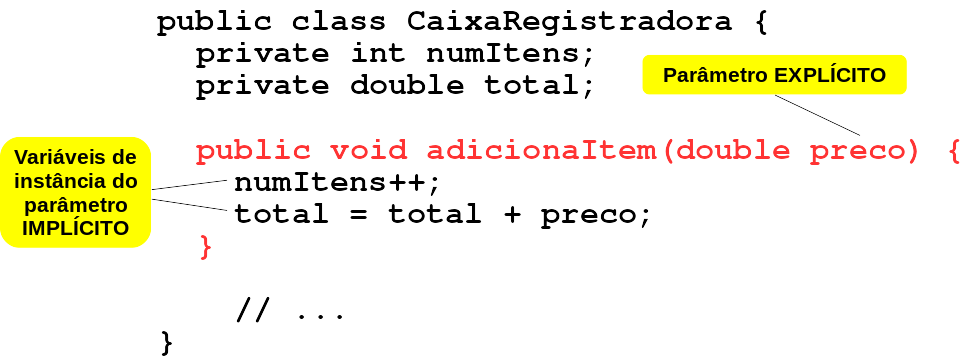
\includegraphics[height=0.60\paperheight,center]{pucrs-ep-fprog-unidade_07-objetos_e_classes-laminas-sintaxe_metodos_de_instancia.png}
\end{figure}
\end{frame}

%-------------------------------------------------------
\begin{frame}\frametitle{Parâmetros Implícitos e Explícitos}
\begin{itemize}
	\item Quando um item é adicionado, isto afeta as variáveis de instância do objeto sobre o qual o método é invocado
\end{itemize}
\begin{figure}[h]
	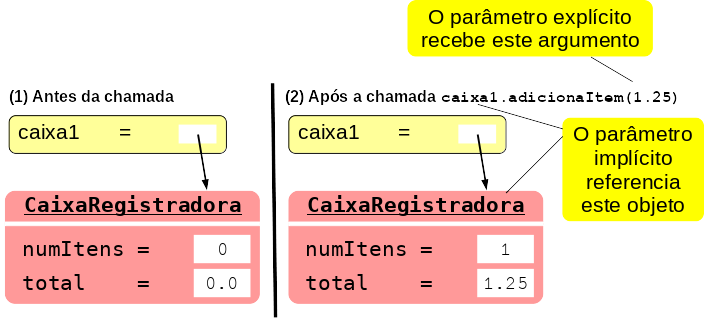
\includegraphics[height=0.60\paperheight,center]{pucrs-ep-fprog-unidade_07-objetos_e_classes-laminas-antes_e_depois_de_uma_chamada.png}
\end{figure}
\end{frame}

%-------------------------------------------------------
\begin{frame}[fragile]\frametitle{Erros Comuns (1)}
\begin{itemize}
	\item Não inicializar referências a objetos na construção
	\begin{itemize}
		\item Referências são inicializadas por padrão com \texttt{null}
		\item Chamar um médoto de uma referência que contém \texttt{null} resulta em um erro de execução: \texttt{NullPointerException}
		\item O compilador consegue apenas detectar variáveis locais não inicializadas, gerando um erro de compilação
	\end{itemize}
\end{itemize}
{\scriptsize
\begin{javacode}
public class ErrosComuns {
  private String nome;  // O construtor default inicializará nome com null

  public void mostraNomes() {
    String nomeLocal;
    // Erro de execução: java.lang.NullPointerException
    System.out.println( nome.length() );
    // Erro de compilação: a variável nomeLocal pode NÃO ter sido inicializada
    System.out.println( nomeLocal.length() );
  }
}
\end{javacode}
}
\end{frame}

%-------------------------------------------------------
\begin{frame}[fragile]\frametitle{Erros Comuns (2)}
\begin{itemize}
	\item Tentar chamar um construtor
	\begin{itemize}
		\item Não se pode chamar um construtor como é feito com outros métodos
		\item Ele é ``invocado'' automaticamente pela palavra reservada \texttt{new}
\begin{javacode}
CaixaRegistradora caixa = new CaixaRegistradora();
\end{javacode}
		\item Não se pode invocar um construtor para um objeto que já existe
\begin{javacode}
caixa.CaixaRegistradora(); // ERRO!
\end{javacode}
		\item Mas pode-se criar um novo objeto usando uma referência existente
\begin{javacode}
CaixaRegistradora caixa = new CaixaRegistradora();
caixa.adicionaItem(1.25);
caixa = new CaixaRegistradora();
\end{javacode}
	\end{itemize}
\end{itemize}
\end{frame}

%-------------------------------------------------------
\begin{frame}[fragile]\frametitle{Erros Comuns (3)}
\begin{itemize}
	\item Declarar um construtor como \texttt{void}
	\begin{itemize}
		\item Construtores não tem tipo de retorno
		\item Isto cria um método com um tipo de retorno \texttt{void} que NÃO é um construtor!
		\item O compilador Java não considera isto um erro...
	\end{itemize}
\begin{javacode}
public class CaixaRegistradora {
  // ...

  /** Pretendia-se criar um construtor... */
  public void CaixaRegistradora() { 
    // ...
  }
}
\end{javacode}
\end{itemize}
\end{frame}

%-------------------------------------------------------
\begin{frame}[fragile]\frametitle{Sobrecarga (\emph{Overloading})}
\begin{itemize}
	\item Pode-se criar múltiplos construtores para uma classe
	\item Cada um deles tem o mesmo nome, mas possui uma lista de parâmetros diferente
	\item Isto se chama \textbf{sobrecarga} e pode ser aplicado a qualquer método em Java
	\begin{itemize}
		\item Sobrecarga = mesmo nome de método com parâmetros diferentes
	\end{itemize}
\begin{javacode}
void imprima(CaixaRegistradora caixa) { ... }
void imprima(ContaBancaria conta)     { ... }
void imprima(int valor)               { ... }
void imprima(double valor)            { ... }
\end{javacode}
\end{itemize}
\end{frame}

%-------------------------------------------------------
\begin{frame}[fragile]\frametitle{\texttt{CaixaRegistradora.java}}
{\tiny\inputminted[bgcolor=cyan!10]{java}{src/caixa2/CaixaRegistradora.java}}
\end{frame}

%-------------------------------------------------------
\begin{frame}[fragile]\frametitle{\texttt{Fruteira.java}}
{\tiny\inputminted[bgcolor=cyan!10]{java}{src/caixa2/Fruteira.java}}
\end{frame}

%-------------------------------------------------------
\begin{frame}[fragile]\frametitle{Exercícios}
\begin{enumerate}
	\item Implemente uma classe chamada \texttt{ContaBancaria} que gerencie os dados de uma conta bancária, considerando as seguintes informações: número da conta (valor inteiro), nome do titular da conta (cadeia de caracteres) e saldo (valor real). Para gerenciar os objetos dessa classe implemente métodos para: construir objetos (considere um construtor que recebe todos os dados e outro que recebe o número da conta e o titular), realizar depósito, realizar saque (considere que o valor do saldo NÃO poderá ser negativo), obter os dados da conta, modificar os dados da conta e obter uma cadeia de caracteres com todos os dados da conta (chame este método de \texttt{toString()}).
	\item Implemente uma classe com método \texttt{main()} para exemplificar o uso da classe \texttt{ContaBancaria}.
\end{enumerate}
\end{frame}

%-------------------------------------------------------
\begin{frame}[fragile]\frametitle{Solução: \texttt{ContaBancaria.java}}
{\tiny\inputminted[bgcolor=cyan!10]{java}{src/conta/ContaBancaria.java}}
\end{frame}

%-------------------------------------------------------
\begin{frame}[fragile]\frametitle{Solução: \texttt{GerenciaContaBancaria.java}}
{\tiny\inputminted[bgcolor=cyan!10]{java}{src/conta/GerenciaContaBancaria.java}}
\end{frame}

\begin{comment}
// exibir menu, obter a entrada, etc.
public Menu();
public void addOption(String option);
public int getInput();
/** Adiciona uma opcao no final deste menu.
    @param option a opcao a ser adicionada
 */
private String[] options;                     private int numOptions;
public void addOption(String option) {
  if (numOptions < options.length) {   options[numOptions++] = option; }  else { ... }
}
\end{comment}

%=======================================================
\section{Testando uma Classe}

%-------------------------------------------------------
\begin{frame}[fragile]\frametitle{Testando uma Classe}
\begin{itemize}
	\item A maioria das classes que os programadores criam não possui método \texttt{main()}, pois elas são criadas para fazer parte de um programa maior
	\item Para testar uma classe será preciso criar um \textbf{teste unitário}
	\item Para testar uma nova classe pode-se usar:
	\begin{itemize}
		\item Ferramentas de programação que criam objetos interativamente:
		\begin{itemize}
			\item DrJava: \url{http://www.drjava.org}
			\item BlueJ: \url{http://www.bluej.org}
		\end{itemize}
		\item Escrever uma classe de teste com um método \texttt{main()}:
\begin{javacode}
public class TestaContaBancaria {
  public static void main(String[] args) {
    ContaBancaria c1 = new ContaBancaria();
    ...
\end{javacode}
	\end{itemize}
\end{itemize}
\end{frame}

%-------------------------------------------------------
\begin{frame}[fragile]\frametitle{Usando BlueJ para Teste}
\begin{itemize}
	\item BlueJ pode instanciar objetos de uma classe interativamente, o que permite que seus métodos sejam invocados
	\item Isto é excelente para realizar testes!
\end{itemize}
\begin{figure}[h]
	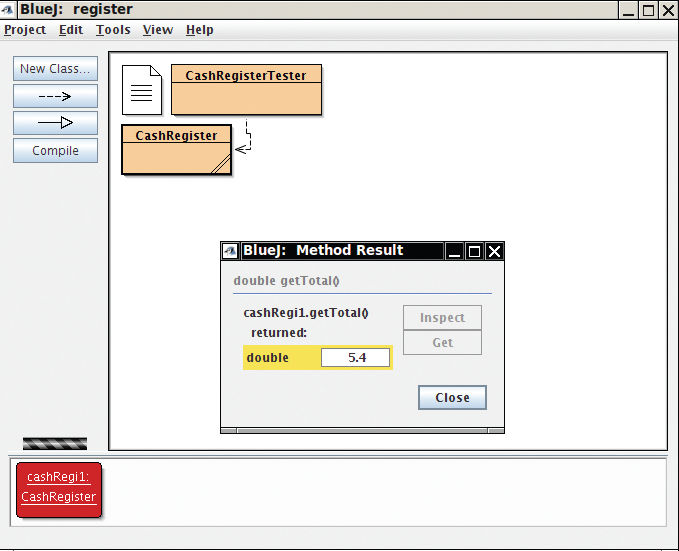
\includegraphics[height=0.55\paperheight,center]{pucrs-ep-fprog-unidade_07-objetos_e_classes-laminas-bluej.jpg}
\end{figure}
\end{frame}

%-------------------------------------------------------
\begin{frame}[fragile]\frametitle{Criando uma Unidade de Teste}
\begin{itemize}
	\item Uma unidade de teste verifica se uma classe funciona corretamente de forma isolada (fora do programa completo)
	\item Ela deve testar todos os métodos, identificando quando alguma inconsistência for identificada
{\tiny\inputminted[bgcolor=cyan!10]{java}{src/caixa2/TestaCaixaRegistradora.java}}
\end{itemize}
\end{frame}

%=======================================================
\section{Padrões para Dados de Objetos}

%-------------------------------------------------------
\begin{frame}\frametitle{Padrões para Dados de Objetos}
\begin{itemize}
	\item Existem alguns padrões comuns quando variáveis de instância são projetadas
	\begin{itemize}
		\item Manter um total
		\item Contar eventos
		\item Coletar valores
		\item Gerenciar propriedades de objetos
		\item Modelar objetos com diferentes estados
		\item Descrever a posição de um objeto
	\end{itemize}
\end{itemize}
\end{frame}

%-------------------------------------------------------
\begin{frame}[fragile]\frametitle{Padrão: Manter um Total}
\begin{columns}[T]
	\begin{column}{0.5\linewidth}
\begin{itemize}
	\item Exemplos
	\begin{itemize}
		\item Total de caixas registradoras
		\item Saldo de contas bancárias
		\item Nível do tanque de gasolina de um carro
	\end{itemize}
	\item Variáveis necessárias
	\begin{itemize}
		\item Total: \texttt{total}
	\end{itemize}
	\item Métodos necessários
	\begin{itemize}
		\item Adição: \texttt{adicionaItem()}
		\item Inicialização: \texttt{limpa()}
		\item Acesso: \texttt{obtemTotal()}
	\end{itemize}
\end{itemize}
	\end{column}
	\begin{column}{0.5\linewidth}
{\scriptsize\inputminted[bgcolor=cyan!10]{java}{src/caixa0/CaixaRegistradora.java}}
	\end{column}
\end{columns}
\end{frame}

%-------------------------------------------------------
\begin{frame}[fragile]\frametitle{Padrão: Contar Eventos}
\begin{columns}[T]
	\begin{column}{0.5\linewidth}
\begin{itemize}
	\item Exemplos
	\begin{itemize}
		\item Número de itens de uma caixa registradora
		\item Custo de transações bancárias
	\end{itemize}
	\item Variáveis necessárias
	\begin{itemize}
		\item Contagem: \texttt{numItens}
	\end{itemize}
	\item Métodos necessários
	\begin{itemize}
		\item Incrementar: \texttt{adicionaItem()}
		\item Inicialização: \texttt{limpa()}
		\item Acesso: \texttt{obtemNumItens()}
	\end{itemize}
\end{itemize}
	\end{column}
	\begin{column}{0.5\linewidth}
{\tiny\inputminted[bgcolor=cyan!10]{java}{src/caixa1/CaixaRegistradora.java}}
	\end{column}
\end{columns}
\end{frame}

%-------------------------------------------------------
\begin{frame}[fragile]\frametitle{Padrão: Colectar Valores}
\begin{columns}[T]
	\begin{column}{0.5\linewidth}
\begin{itemize}
	\item Exemplos
	\begin{itemize}
		\item Carrinho de compras
		\item Questões de múltipla escolha
		\item Placar de pontos
		\item Opções de um menu
	\end{itemize}
	\item Valores armazenados, por exemplo, usando um \emph{array} parcialmente preenchido
	\item Construtor
	\begin{itemize}
		\item Inicializa ou cria a coleção vazia
	\end{itemize}
	\item Métodos necessários
	\begin{itemize}
		\item Adição: \texttt{adicionaItem(), \texttt{obtemNumItens()}, \texttt{obtemItem()}}
	\end{itemize}
\end{itemize}
	\end{column}
	\begin{column}{0.5\linewidth}
{\tiny\inputminted[bgcolor=cyan!10]{java}{src/carrinho/CarrinhoDeCompras.java}}
	\end{column}
\end{columns}
\end{frame}

%-------------------------------------------------------
\begin{frame}[fragile]\frametitle{Padrão: Gerenciar Propriedades de Objetos}
\begin{columns}[T]
	\begin{column}{0.5\linewidth}
\begin{itemize}
	\item Uma propriedade de um objeto pode ser definida e recuperada
	\item Exemplos
	\begin{itemize}
		\item Estudante: matrícula e nome
	\end{itemize}
	\item Construtor
	\begin{itemize}
		\item Inicializa as variáveis de instância
	\end{itemize}
	\item Métodos necessários
	\begin{itemize}
		\item Obtenção: \texttt{obtemMatricula()}, \texttt{obtemNome()}
		\item Definição: \texttt{defineMatricula()}, \texttt{defineNome()}
	\end{itemize}
\end{itemize}
	\end{column}
	\begin{column}{0.5\linewidth}
{\tiny\inputminted[bgcolor=cyan!10]{java}{src/estudante/Estudante.java}}
	\end{column}
\end{columns}
\end{frame}

%-------------------------------------------------------
\begin{frame}[fragile]\frametitle{Padrão: Modelar Objetos com Diferentes Estados}
\begin{columns}[T]
	\begin{column}{0.5\linewidth}
\begin{itemize}
	\item Alguns objetos podem estar em um estado de um conjunto de estados possíveis
	\item Exemplos
	\begin{itemize}
		\item Um peixe que pode estar nos seguintes estados: sem forme, com alguma fome, com muita fome
	\end{itemize}
	\item O peixe inicia sem fome (construtor)	
	\item A fome do peixe é alterada através de
	\begin{itemize}
		\item \texttt{come()}
		\item \texttt{nada()}
	\end{itemize}
	\item Pode-se conferir a fome com \texttt{obtemFome()}
\end{itemize}
	\end{column}
	\begin{column}{0.5\linewidth}
{\tiny\inputminted[bgcolor=cyan!10]{java}{src/peixe/Peixe.java}}
	\end{column}
\end{columns}
\end{frame}

%-------------------------------------------------------
\begin{frame}[fragile]\frametitle{Padrão: Descrever a Posição de um Objeto}
\begin{columns}[T]
	\begin{column}{0.4\linewidth}
\begin{itemize}
	\item Exemplos
	\begin{itemize}
		\item Inseto em uma grade
		\item Objetos de um jogo
		\item Bala de canhão
	\end{itemize}
	\item Valores armazenados
	\begin{itemize}
		\item Linha, coluna, direção, etc.
	\end{itemize}
	\item Métodos necessários
	\begin{itemize}
		\item construtor
		\item \texttt{anda()}
		\item \texttt{gira()}
	\end{itemize}
\end{itemize}
\begin{figure}[h]
	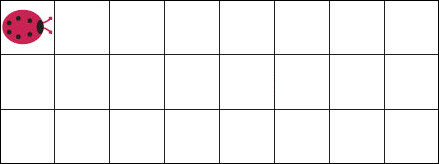
\includegraphics[height=0.16\paperheight,center]{pucrs-ep-fprog-unidade_07-objetos_e_classes-laminas-inseto.jpg}
\end{figure}
	\end{column}
	\begin{column}{0.6\linewidth}
{\tiny\inputminted[bgcolor=cyan!10]{java}{src/inseto1/Inseto.java}}
	\end{column}
\end{columns}
\end{frame}

%-------------------------------------------------------
\begin{frame}[fragile]\frametitle{Exercícios}
\begin{enumerate}
	\item Implemente quatro classes (cada uma com seu método \texttt{main()}) para testar as classes \texttt{CarrinhoDeCompras}, \texttt{Estudante}, \texttt{Peixe} e \texttt{Inseto} (citadas nas 4 lâminas anteriores).\\\scriptsize{~\\Sugestão: na classe \texttt{Inseto}, substitua o método \texttt{toString()} por um método que mostre a grade com o inseto na sua posição e direção corretas (use os caracteres '>', 'v', '<' e '\textasciicircum' para indicar o inseto e sua direção -- use '.' para indicar uma posição vazia da grade).}
\end{enumerate}
\end{frame}

\begin{comment}
%-------------------------------------------------------
\begin{frame}[fragile]\frametitle{Solução: \texttt{SelecionaProdutos.java}}
{\tiny\inputminted[bgcolor=cyan!10]{java}{src/carrinho/SelecionaProdutos.java}}
\end{frame}

%-------------------------------------------------------
\begin{frame}[fragile]\frametitle{Solução: \texttt{GerenciaEstudante.java}}
{\tiny\inputminted[bgcolor=cyan!10]{java}{src/estudante/GerenciaEstudante.java}}
\end{frame}

%-------------------------------------------------------
\begin{frame}[fragile]\frametitle{Solução: \texttt{ControlaPeixe.java}}
{\tiny\inputminted[bgcolor=cyan!10]{java}{src/peixe/ControlaPeixe.java}}
\end{frame}

%-------------------------------------------------------
\begin{frame}[fragile]\frametitle{Solução: \texttt{Inseto.java}}
{\tiny\inputminted[bgcolor=cyan!10]{java}{src/inseto2/Inseto.java}}
\end{frame}

%-------------------------------------------------------
\begin{frame}[fragile]\frametitle{Solução: \texttt{ControlaInseto.java}}
{\tiny\inputminted[bgcolor=cyan!10]{java}{src/inseto2/ControlaInseto.java}}
\end{frame}
\end{comment}

%=======================================================
\section{Referências a Objetos}

%-------------------------------------------------------
\begin{frame}[fragile]\frametitle{Referências a Objetos}
\begin{itemize}
{\small
	\item Uma referência a um objeto especifica a localização de memória do objeto
	\item Objetos são parecidos com \emph{arrays} porque eles também são acessados por referências
\begin{columns}[T]
	\begin{column}{0.6\linewidth}
{\scriptsize
\begin{javacode}
// Referência a array
double[] valores = new double[6];
\end{javacode}
}
	\end{column}
	\begin{column}{0.4\linewidth}
\begin{figure}[h]
	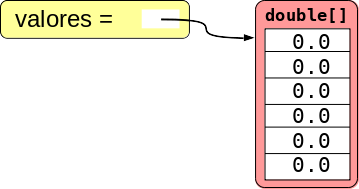
\includegraphics[height=0.25\paperheight,center]{pucrs-ep-fprog-unidade_07-objetos_e_classes-laminas-referencia_a_array.png}
\end{figure}
	\end{column}
\end{columns}
~\\
~\\
\begin{columns}[T]
	\begin{column}{0.6\linewidth}
{\scriptsize	
\begin{javacode}
// Referência a objeto
CaixaRegistradora caixa = new CaixaRegistradora();
\end{javacode}
}
	\end{column}
	\begin{column}{0.4\linewidth}
\begin{figure}[h]
	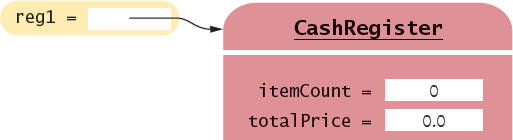
\includegraphics[height=0.15\paperheight,center]{pucrs-ep-fprog-unidade_07-objetos_e_classes-laminas-referencia_a_objeto.png}
\end{figure}
	\end{column}
\end{columns}
	}
\end{itemize}
\end{frame}

%-------------------------------------------------------
\begin{frame}[fragile]\frametitle{Referências Compartilhadas}
\begin{itemize}
{\small
	\item Múltiplas variáveis do tipo objeto podem conter referências para o mesmo objeto.
	\begin{itemize}
{\small
		\item Referência simples
\begin{javacode}
CaixaRegistradora caixa = new CaixaRegistradora();
\end{javacode}
\begin{figure}[h]
	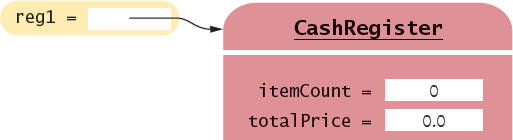
\includegraphics[height=0.10\paperheight,center]{pucrs-ep-fprog-unidade_07-objetos_e_classes-laminas-referencia_a_objeto.png}
\end{figure}
		\item Referências compartilhando o mesmo objeto
\begin{javacode}
CaixaRegistradora aux = caixa;
\end{javacode}
\begin{figure}[h]
	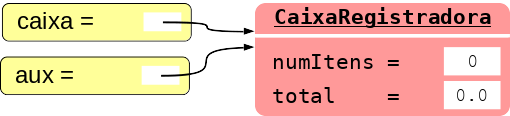
\includegraphics[height=0.10\paperheight,center]{pucrs-ep-fprog-unidade_07-objetos_e_classes-laminas-referencia_a_objeto_2.png}
\end{figure}
}
	\end{itemize}
	\item Os valores internos podem ser alterados através de qualquer uma das referências
}
\end{itemize}
\end{frame}

%-------------------------------------------------------
\begin{frame}[fragile]\frametitle{Cópia de Tipos Primitivos \emph{versus} de Referências}
\begin{itemize}
{\small
	\item Variáveis de tipos primitivos podem ser copiadas, mas funcionam de forma diferente do que referências de objetos
}
\end{itemize}
\begin{columns}[T]
	\begin{column}{0.35\linewidth}
\begin{itemize}
{\scriptsize
	\item Cópia de dados primitivos:\\2 localizações
{\scriptsize
\begin{javacode}
int num1 = 10;
int num2 = num1;
num2++;
\end{javacode}
}
\begin{figure}[h]
	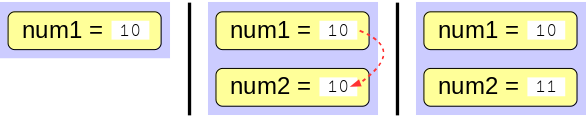
\includegraphics[height=0.11\paperheight,center]{pucrs-ep-fprog-unidade_07-objetos_e_classes-laminas-copia_de_primitivos.png}
\end{figure}
}
\end{itemize}
	\end{column}
	\begin{column}{0.65	\linewidth}
\begin{itemize}
{\scriptsize
	\item Cópia de referências:\\2 referências para a mesma localização
{\scriptsize
\begin{javacode}
CaixaRegistradora caixa = new CaixaRegistradora();
CaixaRegistradora aux = caixa;
aux.adicionaItem(1.25);
\end{javacode}
}
\begin{figure}[h]
	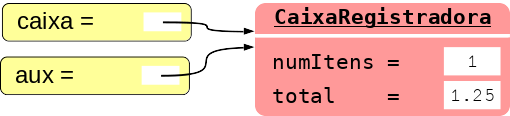
\includegraphics[height=0.14\paperheight,center]{pucrs-ep-fprog-unidade_07-objetos_e_classes-laminas-copia_de_referencias.png}
\end{figure}
	\item Objetos podem ocupar muito mais espaço, por isso Java realiza a cópia apenas da referência
}
\end{itemize}	
	\end{column}
\end{columns}
\end{frame}

%-------------------------------------------------------
\begin{frame}[fragile]\frametitle{A Referência \texttt{null}}
\begin{itemize}
	\item Uma referência pode apontar para ``nenhum'' objeto (\texttt{null})
	\item Não se pode invocar métodos de um objeto através de uma referência \texttt{null}, pois isto causará uma exceção
{\footnotesize
\begin{javacode}
CaixaRegistradora caixa = null;
System.out.println( caixa.obtetmTotal() );   // Erro de execução
\end{javacode}
}
	\item Deve-se testar todas as referência antes de tentar acessá-las:
{\footnotesize
\begin{javacode}
String nomeDoMeio = null; // Nenhum nome do meio

if (nomeDoMeio == null)
  System.out.println( nome + " " + sobrenome );
else
  System.out.println( nome + " " + nomeDoMeio + " " + sobrenome );
\end{javacode}
}
\end{itemize}
\end{frame}

%-------------------------------------------------------
\begin{frame}[fragile]\frametitle{A Referência \texttt{this}}
\begin{itemize}
	\item Métodos recebem um ``parâmetro implícito'' em uma variável de referência chamada \texttt{this}
	\item Trata-se de uma referência ao objeto sobre o qual o método foi invocado:
\begin{figure}[h]
	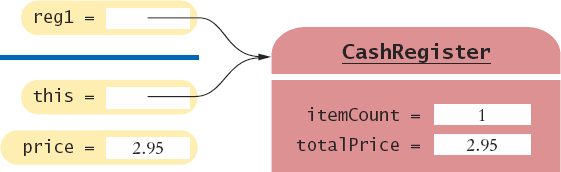
\includegraphics[height=0.2\paperheight,center]{pucrs-ep-fprog-unidade_07-objetos_e_classes-laminas-this.png}
\end{figure}
	\item Assim pode-se deixar mais claro quando será usada uma variável de instância
\begin{javacode}
void adicionaItem(double preco) {
  this.numItens++;
  this.total = this.total + preco;
}
\end{javacode}
\end{itemize}
\end{frame}

%-------------------------------------------------------
\begin{frame}[fragile]\frametitle{Referências a \texttt{this} em Construtores}
\begin{itemize}
	\item A referência \texttt{this} é muito usada em construtores e \emph{setters} (assim variáveis paramétricas e de instância podem ter o mesmo nome)
\begin{javacode}
public class Estudante {
  private int matricula;
  private String nome;
  public Student(int matricula, String nome) {
    this.matricula = matricula;
    this.nome = nome;
  }
}
\end{javacode}
\end{itemize}
\end{frame}

%=======================================================
\section{Variáveis Estáticas e Métodos}

%-------------------------------------------------------
\begin{frame}[fragile]\frametitle{Variáveis e Métodos Estáticos}
\begin{itemize}
	\item Variáveis podem ser declaradas como \texttt{static} na declaração da classe
	\begin{itemize}
		\item Haverá apenas uma cópia da variável \texttt{static} que será compartilhada entre todos os objetos da classe
{\scriptsize
\begin{javacode}
public class ContaBancaria {
  private int numero;
  private String titular;
  private double saldo;
  private static int proximoNumeroDeConta = 1000;

  public ContaBancaria(String t) {
    numero = proximoNumeroDeConta++;
    titular = t;
    saldo = 0.0;
  }
  // ...
}
\end{javacode}
}
	\end{itemize}
	\item Métodos de qualquer objeto da classe podem usar ou alterar o valor de uma variável \texttt{static}
\end{itemize}
\end{frame}

%-------------------------------------------------------
\begin{frame}\frametitle{Usando Variáveis Estáticas}
\vskip-1em
\begin{columns}[T]
	\begin{column}{0.4\linewidth}
\begin{itemize}
	\item Exemplo:
	\begin{itemize}
		\item Cada vez que uma nova conta for criada, a variável \texttt{proximoNumeroDeConta} será incrementada pelo construtor
		\item Acessa-se a variável usando \texttt{NomeDaCasse.nomeDaVariavel}
	\end{itemize}
\end{itemize}
	\end{column}
	\begin{column}{0.6\linewidth}
\begin{figure}[h]
	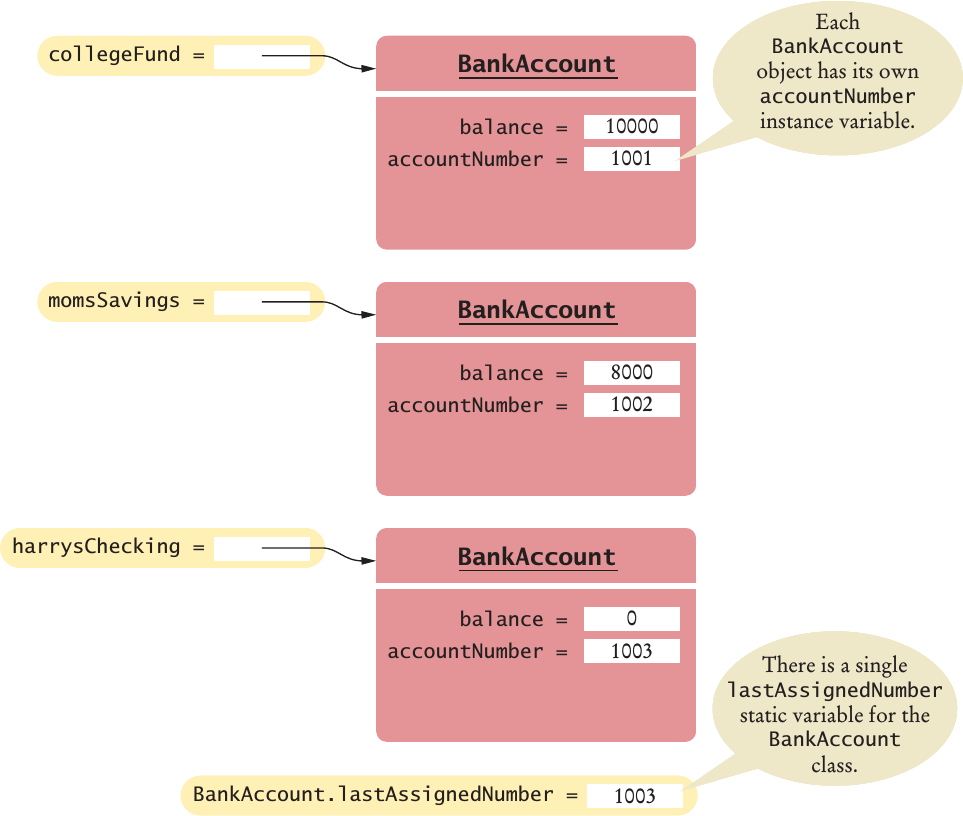
\includegraphics[height=0.7\paperheight,center]{pucrs-ep-fprog-unidade_07-objetos_e_classes-laminas-static.png}
\end{figure}
	\end{column}
\end{columns}
\end{frame}

%-------------------------------------------------------
\begin{frame}[fragile]\frametitle{Usando Métodos Estáticos}
\begin{itemize}
	\item A API de Java tem muitas classes que provêm métodos que podem ser usados sem que se necessite instanciar um objeto
	\begin{itemize}
		\item A classe \texttt{Math} é um bom exemplo disso
		\item Por exemplo, \texttt{Math.sqrt(valor)} é um método estático que retorna a raiz quadrada de um valor
		\item Não é necessário instanciar um objeto da classe \texttt{Math} antes de usá-lo
	\end{itemize}
	\item Métodos \texttt{static} são chamados usando:
\begin{javacode}
NomeDaClasse.nomeDoMetodo();
\end{javacode}
\end{itemize}
\end{frame}

%-------------------------------------------------------
\begin{frame}[fragile]\frametitle{Escrevendo Seus Próprios Métodos Estáticos}
\begin{itemize}
	\item Você pode definir seus próprios métodos estáticos
{\scriptsize
\begin{javacode}
public class Financeiro {
   /** Calcula a porcentagem de determinado valor.
       @param porcentagem A porcentagem a ser aplicada.
       @param quantia A quania sobre a qual a porcentagem será aplicada.
       @return A porcentagem especificada da quantia. */
   public static double percentualDe(double porcentagem, double quantia) {
      return (porcentagem / 100.0) * quantia;
   }
}
\end{javacode}
}
	\item Invoca-se o método estático sobre a classe, e não sobre um objeto
{\scriptsize
\begin{javacode}
double taxa = Financeiro.percentualDe(percentual, total);
\end{javacode}
}
	\item Métodos estáticos geralmente retornam um valor. Eles apenas podem acessar variáveis estáticas e métodos estáticos
\end{itemize}
\end{frame}

%=======================================================
\section{Exercício}

%-------------------------------------------------------
\begin{frame}[fragile]\frametitle{Exercício: Forca}
\begin{itemize}
	\item Implemente uma classe para executar um jogo de Forca (\texttt{Forca.java}) e uma classe para instanciar um objeto desta classe permitindo que o usuário dispute interativamente uma partida de Forca contra o computador (\texttt{App.java}). Pense inicialmente nos métodos que deverão ser chamados para executar o jogo. Implemente um método \texttt{main()} na classe \texttt{App.java} para criar um objeto da classe \texttt{Forca} e executar os métodos desse objeto. A seguir pense nos dados que deverão ser armazenados para cada objeto da classe \texttt{Forca} e implemente-a.
\end{itemize}
\end{frame}

\begin{comment}
%-------------------------------------------------------
\begin{frame}[fragile]\frametitle{Solução: \texttt{App.java}}
{\tiny\inputminted[bgcolor=cyan!10]{java}{src/forca/App.java}}
\end{frame}
\end{comment}

%=======================================================
\section{\emph{Arrays} de Objetos}

%-------------------------------------------------------
\begin{frame}[fragile]\frametitle{\emph{Arrays} de Objetos}
\begin{itemize}
	\item Quando se cria um \emph{array} de algum tipo primitivo, Java preenche todas as posições com um valor nulo (\texttt{0}, \texttt{0.0}, \texttt{false}, etc.)
{\footnotesize
\begin{javacode}
double[] vet = new double[100];
\end{javacode}
}
	\item Quando se cria um \emph{array} de objetos, Java preenche todas as posições com \texttt{null}
{\footnotesize
\begin{javacode}
Classe[] objeto = new Classe[100]; // Nenhum construtor será chamado	
\end{javacode}
}
	\item Isto significa que apenas o \emph{array} foi criado, e NÃO os objetos...
	\item É preciso executar o operador \texttt{new} também para cada um dos objetos
{\footnotesize
\begin{javacode}
for (int i=0; i<objeto.length; ++i)
    objeto[i] = new Classe(); // Agora sim o construtor será chamado
\end{javacode}
}
\end{itemize}
\end{frame}

%=======================================================
\section{Sumário}

%-------------------------------------------------------
\begin{frame}\frametitle{Sumário: Classes e Objetos}
Uma classe descreve um conjunto de objetos com o mesmo comportamento
\begin{itemize}
	\item Cada classe tem uma interface pública: uma coleção de métodos através dos quais os objetos da classe podem ser manipulados
	\item Encapsulamento consiste em prover uma interface pública e esconder os detalhes de implementação
	\item Encapsulamento habilita alterações na implementação sem afetar os usuários da classe
\end{itemize}
\end{frame}

%-------------------------------------------------------
\begin{frame}\frametitle{Sumário: Variáveis e Métodos}
\begin{itemize}
	\item Variáveis de Instância de objetos armazenam dados que são usados pelos seus métodos
	\item Cada objeto de uma classe tem seu próprio conjunto de variáveis de instância
	\item Um método de instância pode acessar variáveis de instância do objeto sobre o qual ele atua
	\item Uma variável de instância privada pode ser acessada apenas por métodos de sua própria classe
	\item Variáveis declaradas como estáticas em uma classe possuem uma única cópia compartilhada entre todos os objetos criados a partir desta classe
\end{itemize}
\end{frame}

%-------------------------------------------------------
\begin{frame}\frametitle{Sumário: Cabeçalhos de Métodos, Dados}
\begin{itemize}
	\item Cabeçalhos de Métodos
	\begin{itemize}
		\item Pode-se usar cabeçalhos de métodos e comentários de métodos para especificar a interface pública de uma classe
		\item Um método \emph{mutator} altera o objeto sobre o qual ele opera
		\item Um método \emph{accessor} não altera o objeto sobre o qual ele atua
	\end{itemize}
	\item Declaração de Dados
	\begin{itemize}
		\item Para cada método \emph{accessor}, um objeto deve ou armazenar ou calcular o resultado
		\item Frequentemente há mais de uma forma de representar os dados de um objeto, e deve-se fazer uma escolha
		\item Deve-se ter certeza de que a representação de dados suporta chamadas de métodos em qualquer ordem
	\end{itemize}
\end{itemize}
\end{frame}

%-------------------------------------------------------
\begin{frame}\frametitle{Sumário: Parâmetros, Construtores}
\begin{itemize}
	\item Parâmetros de Métodos
	\begin{itemize}
		\item O objeto sobre o qual um método é aplicado é o parâmetro implícito
		\item Parâmetros explícitos de um método são listados na declaração do método
	\end{itemize}
	\item Construtores
	\begin{itemize}
		\item Um construtor inicializa as variáveis de instância do objeto
		\item Um construtor é invocado quando um objeto é criado com o operador \texttt{new}
		\item O nome de um construtor é sempre o mesmo que o nome da classe
		\item Uma classe pode ter múltiplos construtores
		\item O compilador seleciona o construtor compatível com os argumentos especificados na criação do objeto
	\end{itemize}
\end{itemize}
\end{frame}

%=======================================================
\section{Tópicos Complementares}

%-------------------------------------------------------
\begin{frame}\frametitle{Depurando Objetos}
\begin{itemize}
	\item Uma sugestão para depurar programas que usam objetos é criar um cartão para cada objeto:
	\begin{itemize}
		\item na parte frontal se apresentam os métodos da interface pública
		\item no verso se controla os dados encapsulados
	\end{itemize}
\end{itemize}
\begin{figure}[h]
	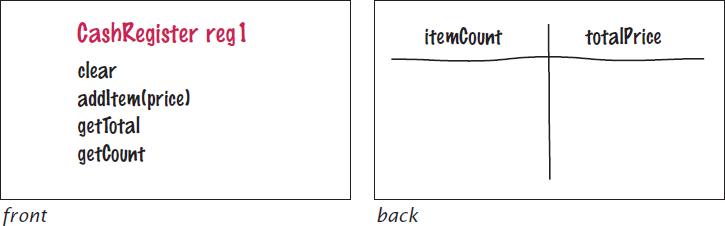
\includegraphics[height=0.40\paperheight,center]{pucrs-ep-fprog-unidade_07-objetos_e_classes-laminas-depurando_objetos.png}
\end{figure}
\end{frame}

%-------------------------------------------------------
\begin{frame}\frametitle{Depurando Objetos (2)}
\begin{itemize}
	\item Quando o construtor for chamado, as variáveis de instância são inicializadas
\begin{figure}[h]
	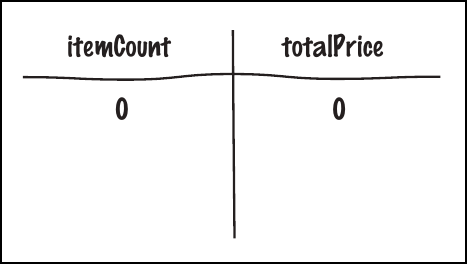
\includegraphics[height=0.25\paperheight,center]{pucrs-ep-fprog-unidade_07-objetos_e_classes-laminas-depurando_objetos_1.png}
\end{figure}
	\item Quando um método \emph{mutator} for chamado, será necessário atualizar variáveis de instância
\begin{figure}[h]
	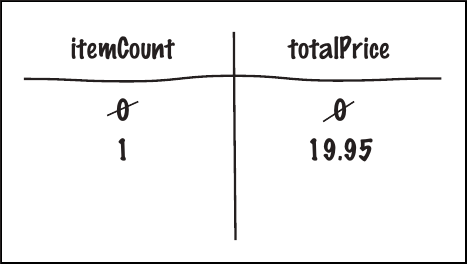
\includegraphics[height=0.25\paperheight,center]{pucrs-ep-fprog-unidade_07-objetos_e_classes-laminas-depurando_objetos_2.png}
\end{figure}
\end{itemize}
\end{frame}

%=======================================================
\section{Referências}

%-------------------------------------------------------
\begin{frame}\frametitle{Referências}
\noindent{HORSTMANN, C. \textbf{Java for Everyone – Late Objects}. 2. ed. Hoboken: Wiley, 2013. xxxiv, 589 p.}
\end{frame}

%=======================================================
\end{document}

